\documentclass[../sparc.tex]{subfiles}
\graphicspath{{\subfix{../images/}}}
\begin{document}

%%%%%%%%%%%%%%%%%%%%%%%%%%%%%%%%%%%%%%%%%%%%%%%%%%%%%%%%%%%%%%%%%%%%%%%%%%%%%%%%
\section{ЖК-дисплей}

Для вывода информации мы будем использовать \emph{жидкокристаллический дисплей}
(ЖК-дисплей), подключаемый к Arduino.  Принцип работы данных дисплеев аналогичен
обычным ЖК-дисплеям, которые выводят информацию на вашем компьютере.  Более
конкретно мы будем использовать \emph{текстовый} ЖК-дисплей, который
предназначен для вывода тестовых символов.

На текстовых ЖК-дисплеях, экран поделён на клетки, внутри каждой из которых
можно отрисовать один символ (букву, знак препинания, цифру, или просто
какую-либо картинку.)  Между клетками обычно находится расстояние в один
пиксель.  Подобные дисплеи плохо подходят для отрисовки произвольных
изображений, тем не менее, некоторый простор для творчества у нас имеется.

Несмотря на свойства дисплея, которые на первый взгляд кажутся слишком
ограничивающими для наших задач, используя наше мастерство и творческий подход,
мы можем добиться достаточно интересных результатов в плане разработки игр.

\subsection{Подключение дисплея}

Для упрощения нашей работы мы будем использовать ЖК-дисплей с интерфейсом
передачи данных, который называется ``I2C'' (читается ``ай-ту-си''.)  Не
вдаваясь в подробности можно сказать, что данный вариант подключения требует
всего 4 провода: питание, земля и две линии передачи данных.

Сам модуль I2C часто уже припаян к дисплею, но может идти и отдельно.  В случае
отдельного модуля, подключение выглядит, как на рис. \ref{fig:lcd-00}.

\begin{figure}[ht]
  \centering
  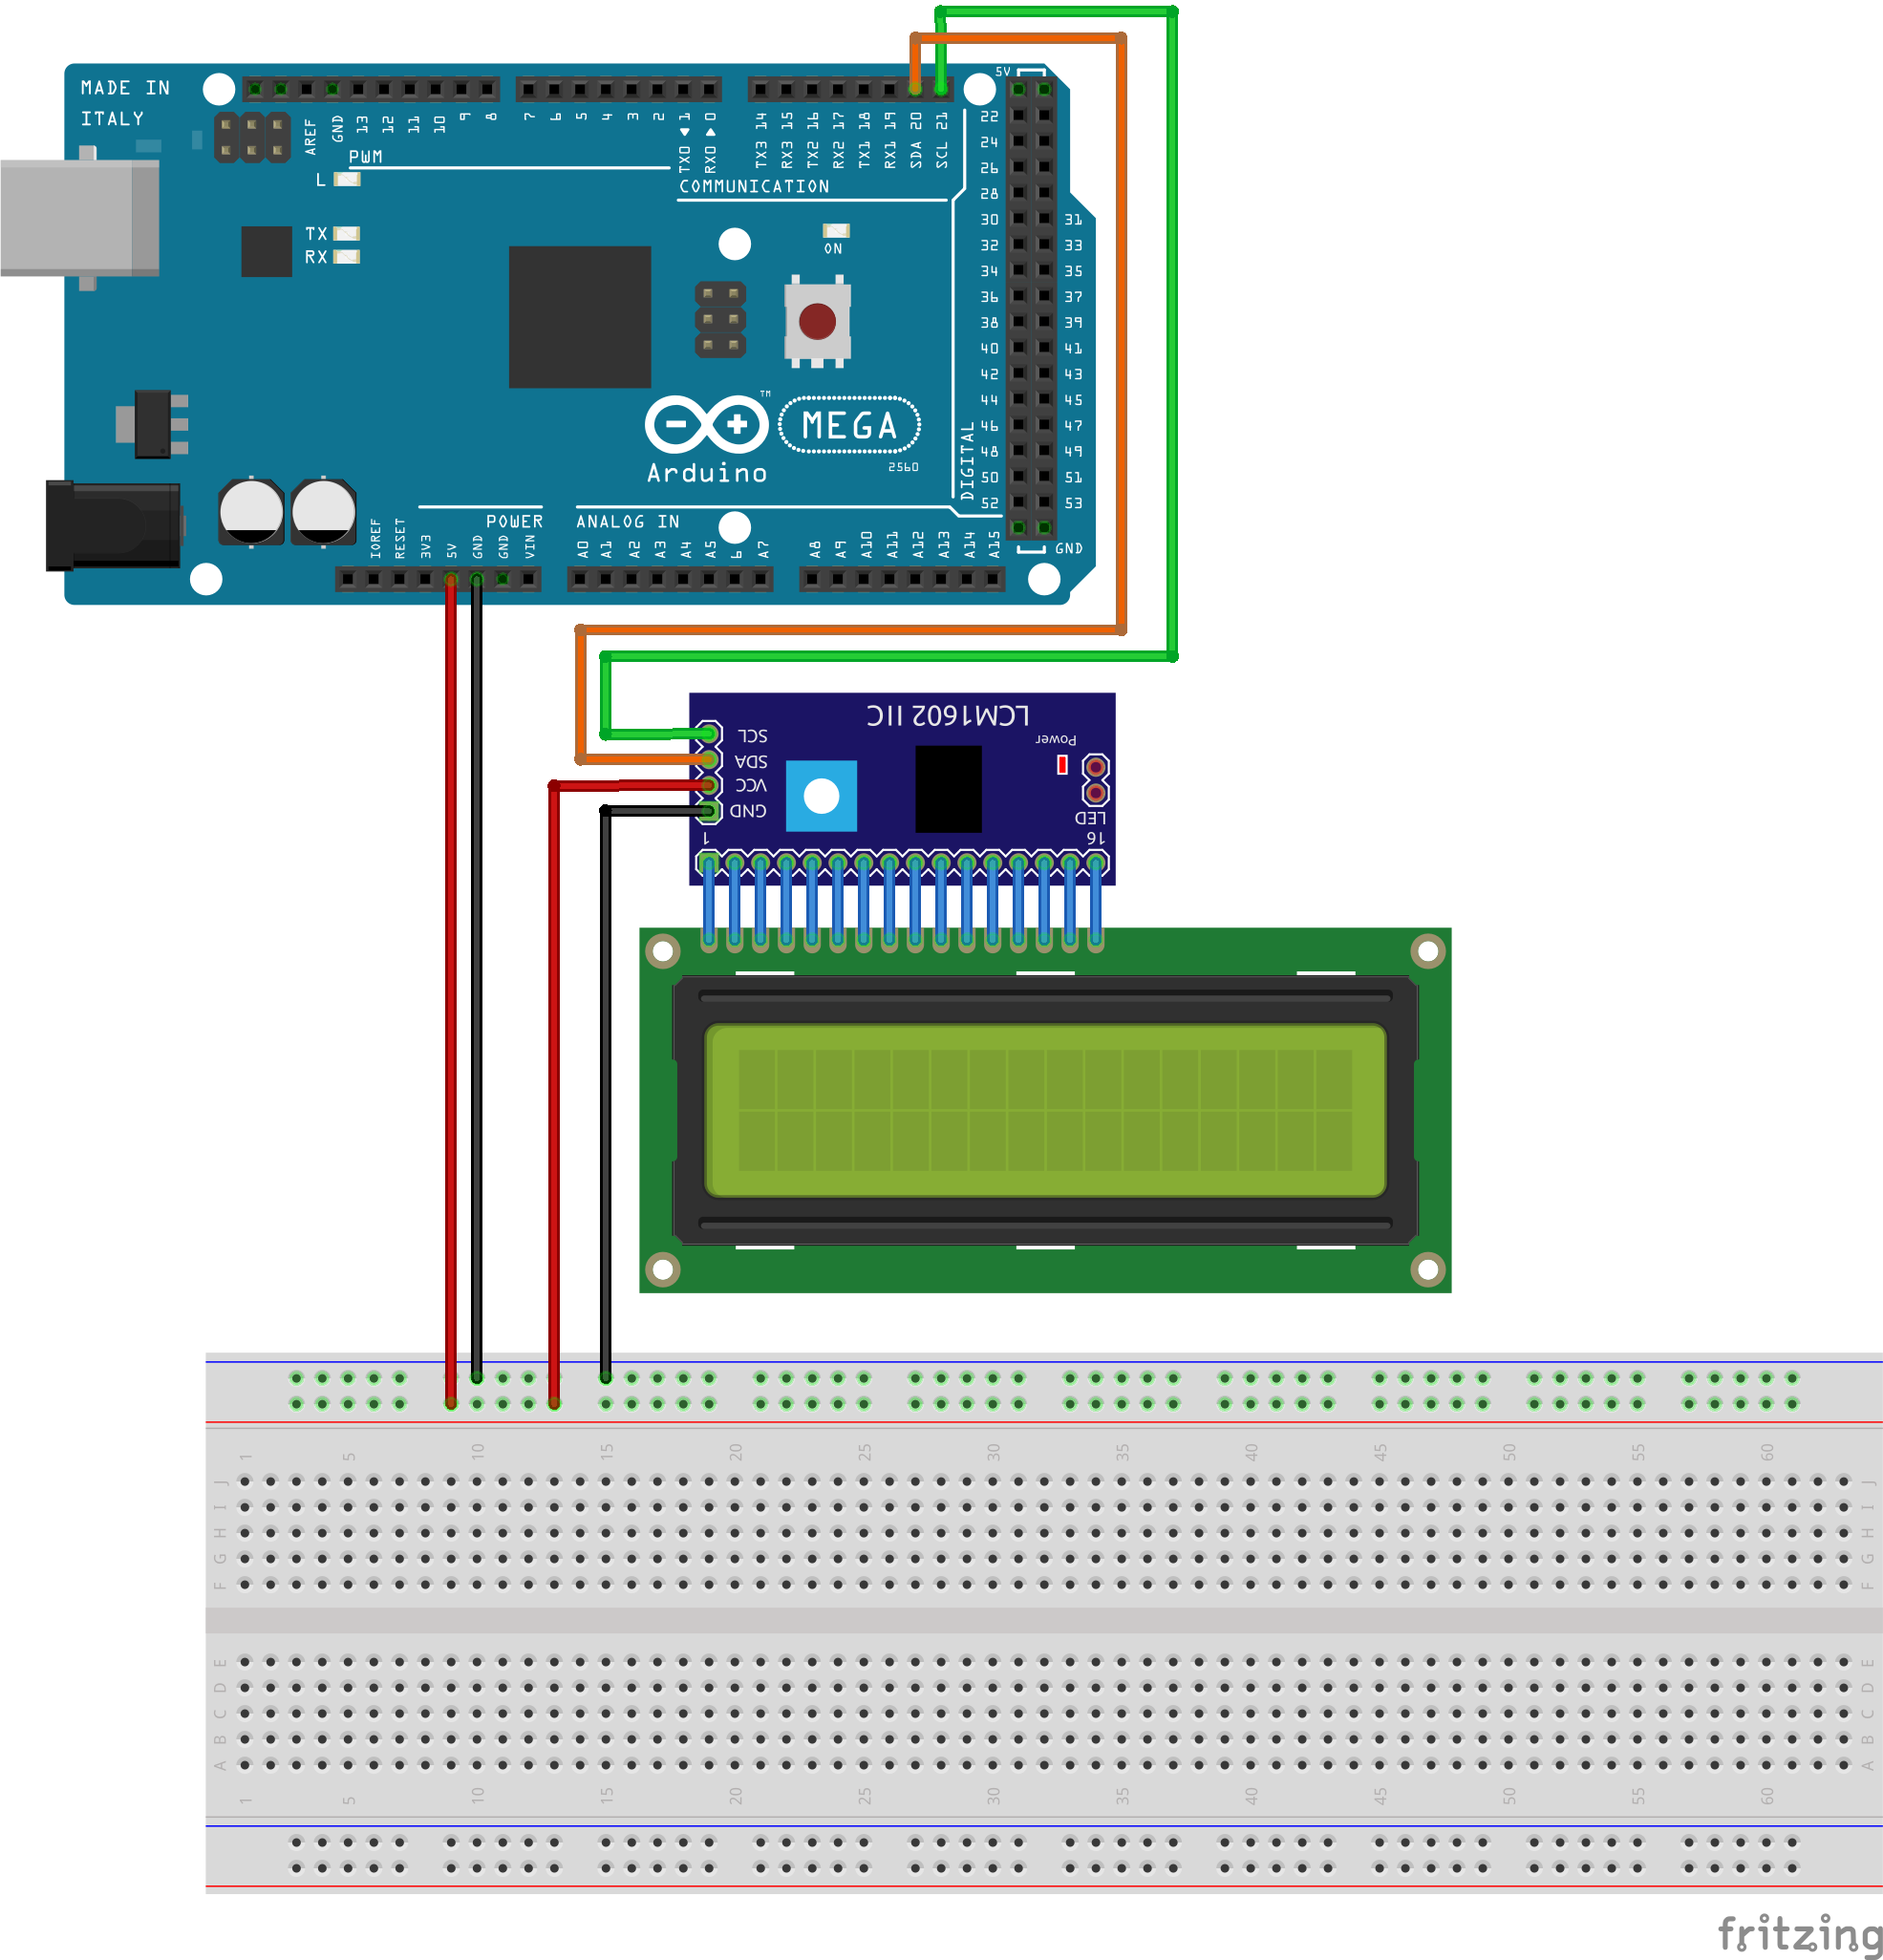
\includegraphics[width=12cm]{schematics/lcd-00}
  \caption{Схема подключения ЖК-дисплея 16x2 по интерфейсу I2C к Arduino Mega
    2560.}
  \label{fig:lcd-00}
\end{figure}

\subsection{Вывод текста}

Согласно традиции, первая программа, которую мы выведем -- это ``Привет, Мир!''.
Однако поскольку вывода русского текста на большинстве дисплеев организован
сложнее, нежели чем латинницы, то мы будем выводить ``Hello, World!''.

Для этого нам необходимо во-первых установить библиотеку для работы с дисплеем;
во-вторых настроить дисплей на нужный режим работы и только после этого мы
сможем вывести текст.

Начнём со скачивания библиотеки.

\end{document}
